\chapter{三维渲染}

计算机图形学的一个基本任务就是三维场景的渲染(Redering)。渲染是指,对于一系列排列在三维空间中的物体,产生一张从三维空间特定视角观察这些物体的二维图像。本质上说,渲染是一系列物体为输入以一个像素阵列为输出的过程,无论具体如何实现,渲染总会涉及到这样一个问题:每个物体是如何影响每个像素的?渲染有以下两种的主流的实现方式
\begin{itemize}
    \item 物体顺序渲染(Object Order Redering),代表技术为光栅化(Raterization)。
    \item 图像顺序渲染(Image Order Redering),代表技术为光线追踪(Ray Tracing)。
\end{itemize}

\begin{Figure}[Ray Tracing In One Weekend]
    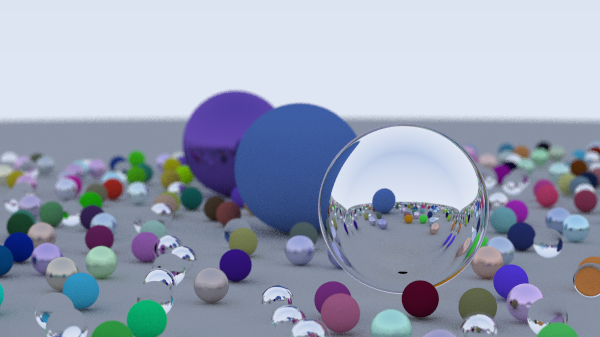
\includegraphics[width=11cm]{image/Final.png}
\end{Figure}

光栅化可以大致分为以下几步
\begin{itemize}
    \item 视角变换:根据观察方向,将三角面的顶点坐标从三维空间变换至二维屏幕。
    \item 光栅化:计算二维屏幕上的每个三角形应当占用哪些像素。
    \item 表面着色:计算出每个三角面在光照下的颜色。
    \item 纹理映射:计算出每个三角面上应呈现的纹理图案(如果有纹理的话)。
\end{itemize}
需要特别指出的是,光栅化既是整个物体顺序渲染过程的名称,亦是其中一个小步骤的名称。\goodbreak

光栅化的优势在于渲染效率较高,事实上,目前主流的GPU和3D游戏都是基于光栅化的三维渲染技术。然而,这种简单的变换虽然可以正确呈现三维场景,但效果往往不够逼真。

\begin{Figure}[NVDIA Fermi架构]
    \includegraphics[scale=0.7]{build/Chapter01A_01.fig.pdf}
    \includegraphics[scale=0.7]{build/Chapter01A_02.fig.pdf}
\end{Figure}

光线追踪是与光栅化相对应的技术,它模拟了现实中的光线行为。其基本思想是,对于图像中的每一像素,向特定方向发出一条光线,该光线会在场景中的物体间发生多次反射和折射,最终到达光源。该像素的颜色就会由其发出光线经过的物体颜色和光源颜色决定。光线追踪可以轻易的实现许多复杂的光学效果,例如:透明材料、反光材料、软阴影、镜头虚化。这是光栅化无法匹敌的,然而,由于光线追踪需要迭代计算光线的传播行为,其效率也相对较低。